\section{Geometrija na ravnini in v prostoru}

\begin{frame}
    \sectionpage
\end{frame}

\begin{frame}
    \tableofcontents[currentsection, hideothersubsections]
\end{frame}

    \subsection{Osnovni geometrijski pojmi}

        \begin{frame}
            \frametitle{Osnovni geometrijski pojmi}
        \end{frame}

    \subsection{Kot}

        \begin{frame}
            \frametitle{Kot}
        \end{frame}

    \subsection{Konstrukcije matematičnih objektov}

        \begin{frame}
            \frametitle{Konstrukcije matematičnih objektov}
        \end{frame}

    \subsection{Preslikave na ravnini}

        \begin{frame}
            \frametitle{Preslikave na ravnini}

            \large\textbf{Pravokotna projekcija}
            ~\\
            ~\\

            \normalsize
            \begin{columns}
                \column{0.60\textwidth}
                    Dani sta točka $T$ in premica $p$. Naj bo $q$ tista pravokotnica na premico $p$, ki poteka skozi točko $T$. 
                    Presečišče $T'$ premice $q$ s premico $p$ imenujemo \textbf{pravokotna projekcija} točke $T$ na premico $p$. 
                    Točka $T'$ je točki $T$ najbližja točka premice $p$. \\
                    ~\\
                    \textbf{Razdalja} točke $T$ od premice $p$ je: $d(T,p)=\left\lvert TT'\right\rvert$.
                \column{0.35\textwidth}            
                    \begin{figure}
                    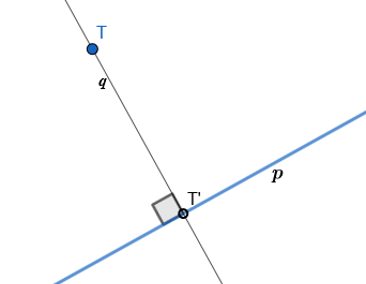
\includegraphics[scale=0.5]{Slike in skice/Pravokotna_projekcija.png}
                    \end{figure}
            \end{columns}
            
        \end{frame}

        \begin{frame}
            \large\textbf{Toge preslikave}
            ~\\
            ~\\
            \normalsize
                Preslikave v ravnini, ki ohranjajo razdaljo so \textbf{toge preslikave}.
                $$d(A,B)=d(A',B')$$

                Med toge preslikave spadajo:
                \begin{itemize}
                    \item \textbf{vzporedni premiki};
                    \item \textbf{zrcaljenje preko premice};
                    \item \textbf{zrcaljenje preko točke};
                    \item \textbf{rotacija okoli točke}.
                \end{itemize}

                ~\\
                Če kombiniramo več togih premikov, je dobljena preslikava spet togi premik.

        \end{frame}

        \begin{frame}
            \large\textbf{Vzporedni premik/translacija}
            ~\\
            ~\\
            \normalsize
            \textbf{Vzporedni premik} ali \textbf{translacija} za usmerjeno daljico (vektor) $\overrightarrow{AB}$ preslika točko $T$ v tako točko $T'$, da sta daljici $TT'$ in $AB$ enako dolgi, vzporedni in enako usmerjeni (vektorja $\overrightarrow{TT'}$ in $\overrightarrow{AB}$ sta enaka). \\
            
            \begin{figure}
                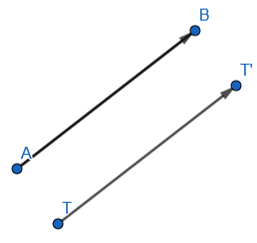
\includegraphics[scale=0.5]{Slike in skice/Vzporedni_premik_tocke.png}
                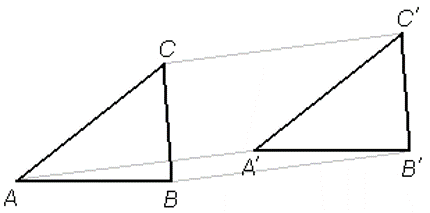
\includegraphics[scale=0.5]{Slike in skice/Vzporedni_premik_trikotnika.png}
            \end{figure}

            Vzporedni premik ohranja orientacijo likov, daljice preslika v enako dolge vzporedne daljice, ohranja velikost kotov, like preslika v skladne like, nima negibnih točk za $\overrightarrow{MN}\neq \overrightarrow{0}$.

        \end{frame}

        \begin{frame}
            \large\textbf{Zrcaljenje preko premice}
            ~\\
            ~\\
            \normalsize
            \textbf{Zrcaljenje čez premico} $p$ preslika točko $T$ v tako točko $T'$, da premica $p$ pod pravim kotom razpolavlja daljico $TT'$.
            
            \begin{figure}
                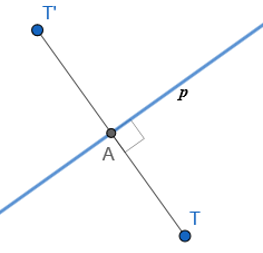
\includegraphics[scale=0.5]{Slike in skice/Zrcaljenje_tocke_cez_premico.png}
                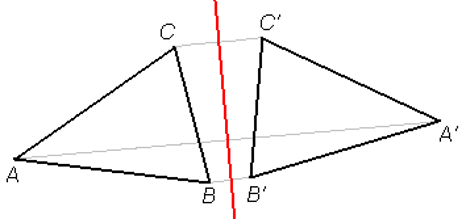
\includegraphics[scale=0.5]{Slike in skice/Zrcaljenje_lika_cez_premico.png}
            \end{figure}

            Zrcaljenje čez premico daljice preslika v enako dolge daljice, ohranja velikost kotov, ne ohranja orientacije likov, like preslika v skladne like, premic ne preslika v vzporedne premice.

        \end{frame}

        
        \begin{frame}
            \large\textbf{Zrcaljenje preko točke}
            ~\\
            ~\\
            \normalsize
            \textbf{Zrcaljenje čez točko} $O$ preslika točko $T$ v tako točko $T'$, da je $O$ razpolovišče daljice $TT'$. Ta preslikava je enaka vrtenju okrog točke za $180^\circ$.

            \begin{figure}
                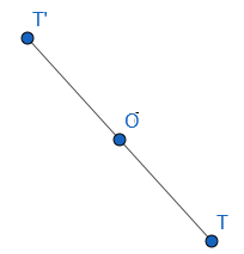
\includegraphics[scale=0.5]{Slike in skice/Zrcaljenje_tocke_cez_tocko.png}
                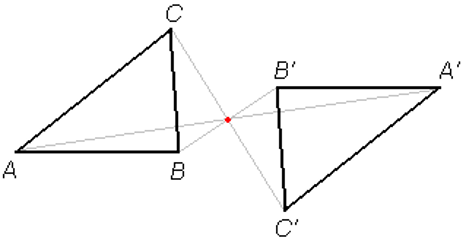
\includegraphics[scale=0.5]{Slike in skice/Zrcaljenje_lika_cez_tocko.png}
            \end{figure}

            Zrcaljenje čez točko daljice preslika v enako dolge daljice, ohranja velikosti kotov in orientacijo likov, like preslika v skladne like, premice preslika v vzporedne premice.

        \end{frame}


        \begin{frame}
            \large\textbf{Rotacija/vrtenje okoli točke}
            ~\\
            ~\\
            \normalsize
            \textbf{Vrtenje} ali \textbf{zasuk} oziroma \textbf{rotacija} za kot $\alpha$ okrog točke $O$ preslika točko $T$ v točko $T'$, da velja: $\left\lvert OT\right\rvert = \left\lvert OT'\right\rvert$  in $\angle TOT' = \alpha$.


            \begin{figure}
                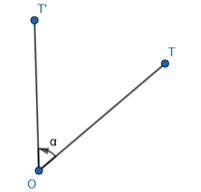
\includegraphics[scale=0.6]{Slike in skice/Rotacija tocke_okoli_tocke.png}
                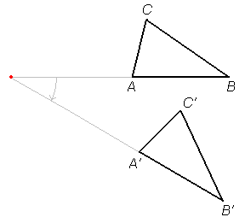
\includegraphics[scale=0.6]{Slike in skice/Rotacija_lika_okoli_tocke.png}
            \end{figure}

        \end{frame}

        \begin{frame}
            
            Če smo kot  odmerili v smeri, ki je nasprotna smeri vrtenja urinega kazalca, smo točko $T$ zavrteli v \textbf{pozitivni smeri} za kot $\alpha$, sicer pa v \textbf{negativni smeri}. 
            Namesto smeri vrtenja lahko usmerimo kot: vrtenju v pozitivni smeri ustreza \textbf{pozitivni kot}, vrtenju v negativni smeri pa \textbf{negativni kot}. \\
            ~\\

            Vrtenje okoli točke preslika daljice v enako dolge daljice, ohranja velikosti kotov in orientacijo likov, like preslika v skladne like, premice pa ne preslika v vzporedne premice. 

        \end{frame}


        \begin{frame}
            \large\textbf{Simetrija}
            ~\\
            ~\\
            \normalsize

            Množica točk $\mathcal{M}$ je \textbf{simetrična/somerna glede na premico} $p$, če se pri zrcaljenju čez premico $p$ preslika sama vase. Premico $p$ imenujemo \textbf{simetrala} (somernica, simetrijska os) množice $\mathcal{M}$. \\
            ~\\
            
            Množica točk $\mathcal{M}$ je (središčno) \textbf{simetrična/somerna glede na točko} $T$, če se pri zrcaljenju čez točko $T$ preslika sama vase. Točko $T$ imenujemo \textbf{center simetrije} množice $\mathcal{M}$. 
            \begin{figure}
                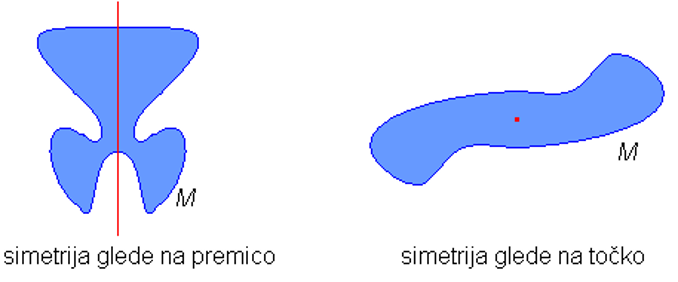
\includegraphics[scale=0.45]{Slike in skice/Simetrija.png}
            \end{figure}

        \end{frame}

    \subsection{Trikotnik}

        \begin{frame}
            \frametitle{Trikotnik}


        \end{frame}

    \subsection{Krog}

        \begin{frame}
            \frametitle{Krog}
        \end{frame}

    \subsection{Štirikotnik}

        \begin{frame}
            \frametitle{Štirikotnik}
        \end{frame}

    \subsection{Večkotnik}

        \begin{frame}
            \frametitle{Večkotnik}
        \end{frame}

    \subsection{Podobnost}

        \begin{frame}
            \frametitle{Podobnost}
        \end{frame}

    \subsection{Podobnost v pravokotnem trikotniku}
        
        \begin{frame}
            \frametitle{Podobnost v pravokotnem trikotniku}
        \end{frame}

    \subsection{Kotne funkcije kotov, velikih od $0^\circ$ do $90^\circ$}
        
        \begin{frame}
            \frametitle{Kotne funkcije kotov, velikih od $0^\circ$ do $90^\circ$}
        \end{frame}
        
    \subsection{Kotne funkcije kotov, velikih od $0^\circ$ do $160^\circ$}
        
        \begin{frame}
            \frametitle{Kotne funkcije kotov, velikih od $0^\circ$ do $360^\circ$}
        \end{frame}
